\documentclass[twoside,a4paper,openright,12pt]{book}


\usepackage[pdftex]{graphicx}
\usepackage{pdfpages}
\usepackage{float}
\usepackage{amsmath}
\usepackage{amssymb}
\usepackage{textcomp}
\usepackage[utf8]{inputenc}
\usepackage[polish]{babel}
\usepackage[T1]{fontenc}
\usepackage{array}
% pakiet stosowany do url'i w bibliografii, zamienia odnośniki na ładnie sformatowane
\usepackage{url}
% pakiety służące do numerowania i tworzenia algorytmów
\usepackage{algorithmic}
\usepackage{algorithm}


% redefinicja etykiety nagłówkowej listy algorytmów, domyślna jest po angielsku
\renewcommand{\listalgorithmname}{Spis algorytmów}

% pakiet do wyliczania skali, przydatny przy dużych obrazkach
\usepackage{pgf}

% pakiet służący do automatycznego sortowania odnośników do bibliografii
%\usepackage[sort]{natbib}

% tworzenie listingów
\usepackage{listings}
\usepackage{color}
\definecolor{lightgray}{rgb}{.9,.9,.9}
\definecolor{darkgray}{rgb}{.4,.4,.4}
\definecolor{purple}{rgb}{0.65, 0.12, 0.82}

\lstdefinelanguage{JavaScript}{
  keywords={typeof, new, true, false, catch, function, return, null, catch, switch, var, if, in, while, do, else, case, break},
  keywordstyle=\color{blue}\bfseries,
  ndkeywords={class, export, boolean, throw, implements, import, this},
  ndkeywordstyle=\color{darkgray}\bfseries,
  identifierstyle=\color{black},
  sensitive=false,
  comment=[l]{//},
  morecomment=[s]{/*}{*/},
  commentstyle=\color{purple}\ttfamily,
  stringstyle=\color{red}\ttfamily,
  morestring=[b]',
  morestring=[b]"
}

\lstset{
   language=JavaScript,
   backgroundcolor=\color{white},
   extendedchars=true,
   basicstyle=\footnotesize\ttfamily,
   showstringspaces=false,
   showspaces=false,
   numbers=left,
   numberstyle=\footnotesize,
   numbersep=9pt,
   tabsize=2,
   breaklines=true,
   showtabs=false,
   captionpos=b
}

% tworzenie figur wewnątrz figur
\usepackage{subfig}

% do automatycznego skracania nazw rozdziałów i podrozdziałów używanych w nagłówkach strony by mieściły się w jednej linii
\usepackage[fit]{truncate}

% fancyhdr - ładne nagłówki, definicja wyglądu nagłówka, numery stron będą umieszczane w nagłówku po odpowiedniej stronie
\usepackage{fancyhdr}
\pagestyle{fancy}
\renewcommand{\chaptermark}[1]{\markboth{#1}{}}
\renewcommand{\sectionmark}[1]{\markright{\thesection\ #1}}
\fancyhf{}
\fancyhead[LE,RO]{\bfseries\thepage}
% tutaj ograniczamy szerokość pola w nagłówku zawierającego nazwę rozdziału/podrozdziału do 95% szerokości strony
% redefinicja sposobu prezentacji nazw domyślnie wypisywanych wielkimi literami (np. domyślnie w nagłówku Spis treści będzie miał postać SPIS TREŚCI)
% Uwaga! to może popsuć wielkie litery w ogóle! Jak coś nie działa należy usunąć \nouppercase{} z poniższych definicji
\fancyhead[LO]{\nouppercase{\bfseries{\truncate{.95\headwidth}{\rightmark}}}}
\fancyhead[RE]{\nouppercase{\bfseries{\truncate{.95\headwidth}{\leftmark}}}}
\renewcommand{\headrulewidth}{0.5pt}
\renewcommand{\footrulewidth}{0pt}

% definicja typu prostego wymagana przez pierwsze strony rozdziałów itp.
% powyższe reguły niestety tych stron nie dotyczą, gdyż Latex automatycznie przełącza je pomiędzy fancy a plain
% w tym wypadku eliminujemy nagłówki i stopki na stronach początkowych
\fancypagestyle{plain}{%
 \fancyhead{}
 \fancyfoot{}
 \renewcommand{\headrulewidth}{0pt}
 \renewcommand{\footrulewidth}{0pt}
}

\parskip 0.05in


% makro umożliwiające otaczanie symboli okręgami
\usepackage{tikz}
% brak justowania tekstu (bazą okręgu będzie linia tekstu)
\newcommand*\mycirc[1]{%
  \begin{tikzpicture}
    \node[draw,circle,inner sep=1pt] {#1};
  \end{tikzpicture}}

% pionowe justowanie tekstu, środek okręgu pokrywa się ze środkiem tekstu
\newcommand*\mycircalign[1]{%
  \begin{tikzpicture}[baseline=(C.base)]
    \node[draw,circle,inner sep=1pt](C) {#1};
  \end{tikzpicture}}

% zmiana nazwy twierdzeń i lematów
\newtheorem{theorem}{Twierdzenie}[section]
\newtheorem{lemma}[theorem]{Lemat}

% tworzenie definicji dowodu
\newenvironment{proof}[1][Dowód]{\begin{trivlist}
\item[\hskip \labelsep {\bfseries #1}]}{\end{trivlist}}
% \newenvironment{definition}[1][Definicja]{\begin{trivlist}
% \item[\hskip \labelsep {\bfseries #1}]}{\end{trivlist}}
% \newenvironment{example}[1][Przykład]{\begin{trivlist}
% \item[\hskip \labelsep {\bfseries #1}]}{\end{trivlist}}
% \newenvironment{remark}[1][Uwaga]{\begin{trivlist}
% \item[\hskip \labelsep {\bfseries #1}]}{\end{trivlist}}

% definicja czarnego prostokąta zwyczajowo dodawanego na koniec dowodu
\newcommand{\qed}{\nobreak \ifvmode \relax \else
      \ifdim\lastskip<1.5em \hskip-\lastskip
      \hskip1.5em plus0em minus0.5em \fi \nobreak
      \vrule height0.75em width0.5em depth0.25em\fi}

% poniższymi instrukcjami można sterować co ma być numerowane a co nie i co ma być wyświetlane w spisie treści
% \setcounter{secnumdepth}{3}
% \setcounter{tocdepth}{5}

% definicja czcionki mniejszej niż tiny (domyślnie takiej małej nie ma)
\usepackage{lmodern}
\makeatletter
  \newcommand\tinyv{\@setfontsize\tinyv{4pt}{6}}
\makeatother

% definicja jeszcze mniejszej czcionki
\usepackage{lmodern}
\makeatletter
  \newcommand\tinyvv{\@setfontsize\tinyvv{3.5pt}{6}}
\makeatother

% pakiet do obsługi wielostronicowych tabel
\usepackage{longtable}
\setlength{\LTcapwidth}{\textwidth}

\usepackage[section] {placeins}

\usepackage{multirow}

\usepackage{slantsc}


% korekta marginesów - domyślnie latex ma jakieś kosmiczne
\usepackage{anysize}
\marginsize{3.5cm}{2.5cm}{2.5cm}{2.5cm}
% po zmianie marginesów konieczne jest wymuszenie przeliczenia nagłówków
\fancyhfoffset[E,O]{0pt}

\renewcommand\lstlistlistingname{Listingi kodu}

\begin{document}

%wyłącznie numerowania stron
\pagenumbering{gobble}

% wklejenie strony tytułowej z oddzielnego PDFa

\includepdf[pages={1}]{StronaTytulowa.pdf}

% sekcja wstępna książki, numerowana rzymskimi
\frontmatter

% dodatkowy, nienumerowany rozdział na np. podziękowania
\chapter*{Podziękowania}

Pragnę podziękować mojemu Promotorowi za wsparcie merytoryczne i motywację, a także najbliższym mi osobom, za doping, wiarę w moje możliwości oraz wyrozumiałość, kiedy nie mogłem poświęcać Im tyle czasu, ile bym chciał.

Dziękuję również wszystkim zainteresowanym osobom, które wypytywały mnie o szczegóły techniczne i postępy tej pracy. Dzięki Wam mogłem lepiej zrozumieć mój projekt.
\addcontentsline{toc}{chapter}{Podziękowania}

% spis treści
\tableofcontents


% właściwa część książki, numerowana arabskimi od 1
\mainmatter

\chapter{Wstęp}
\section{Idea pracy dyplomowej}

Niniejsza praca opisuje projekt i wykonanie mobilnego systemu komunikacji przeznaczonego dla Ośrodków Szkolenia Kierowców roboczo nazwanego ,,OSK-Helper''. Jego architekturę, część wizualną interfejsów, sposób instalacji i~uruchomienia, zalecane przypadki użycia oraz opracowane lub wykorzystane algorytmy.


\section{Założenia projektu}

Głównym założeniem projektu było stworzenie prostej aplikacji mobilnej, która będzie przyjazna dla użytkowników, a jednocześnie nadal będzie spełniała swoje zadanie - ułatwiała komunikacji pomiędzy instruktorami Ośrodków Szkolenia Kierowców w celu zmniejszenia kolizji zajętości placów manewrowych.

Kolejnym założeniem było wykorzystanie języka JavaScript w każdej płaszczyźnie aplikacji, zarówno klienta, jak i serwera oraz użycie nierelacyjnej bazy danych, która będzie przechowywała dane o strukturze zbliżonej do struktury obiektów tego języka.


\section{Cel pracy}

Celem pracy jest projekt i realizacja systemu mającego za zadanie ułatwić pracę instruktorów Prawa Jazdy poprzez zautomatyzowanie wymiany informacji dotyczącej zajętości placów manewrowych, z których mogą korzystać.


\section{Zakres pracy}

Projekt praktyczny, stworzony dla celów niniejszej pracy jest znaczną częścią trudu włożonego w jej powstanie i w jego skład wchodzi:

\begin{itemize}
	\item aplikacja mobilna dla systemu Android
	\item aplikacja serwerowa będąca zapleczem dla mobilnego systemu.
\end{itemize}




\chapter{Wykorzystywane technologie}

\section{JavaScript}

JavaScript jest prototypowym obiektowym językiem programowania. Jest to język Internetu, ze względu na to, że jego kod potrafi uruchomić prawie każda przeglądarka internetowa. Po ciężkim okresie, kiedy to został ogólnie przyjęty jako zabawka umożliwiająca tworzenie tzw. wodotrysków na stronach WWW, rozrósł znacząco i dzisiaj jest jednym z najpopularniejszych, a na pewno najsłynniejszym spośród internetowych języków programowania.

Dzisiejszą ,,Dobę Internetu'' pełną technologii AJAX, rozbudowanych klienckich aplikacji internetowych przypominających desktopowe m.in. czytników RSS, aplikacji biurowych, klientów pocztowych, interaktywnych map, programów do obróbki grafiki i wideo etc. do historii odeszły długotrwałe wywołania stron wykonywane przy każdym wejściu użytkownika  w interakcję z przeglądarką. To wszystko możemy zawdzięczać głównie dzięki JavaScriptowi.

Początkowe wersje interpreterów JavaScript zostały osadzone w jednych z pierwszych wersji przeglądarek Netscape i Internet Explorer. Ta kliencka wersja JavaScriptu pozwala na umieszczanie wykonywalnej zawartości w stronach internetowych, co pozwala na budowanie interakcji z użytkownikiem, to coś więcej niż statyczne strony WWW. Skrypty języka JavaScript odpowiedzialne są za część zachowawczą stron, kiedy to HTML (ang. HyperText Markup Language) opisuje zawartość i strukturę DOM (ang. Document Object Model) oraz treść, a CSS (ang. Cascading Style Sheets) opisuje wygląd tych elementów.

JavaScript jest otwartym standardem, ale standaryzacją tego języka zajmuje się ECMA International (ang. ang. European Computer Manufacturers Association), która na jego podstawie wydała standard języka skryptowego o nazwie ECMAScript, którego już niedługo szósta wersja wprowadzić ma nowe mechanizmy obiektowości, takie jak np. pełnowymiarowe dziedziczenie za pomocą klas (które dzisiaj jest realizowane przez prototypowanie obiektów), modularyzację i hermetyzację (które dzisiaj są realizowane przez zewnętrzne biblioteki wprowadzające tego typu abstrakcje), a także wiele innych usprawnień, które zapewne przyciągną jeszcze większe rzesze programistów na całym świecie.

Obecnie przeglądarki WWW to nie jedyne interpretery w obrębie których możliwe jest uruchomienie kodu JavaScript. Można tworzyć kod do zastosowań po stronie serwera WWW (m.in .NET lub Node.js), skrypty i aplikacje wiersza poleceń CLI (ang. Command Line Interface), aplikacje desktopowe (Node-webkit, Alchemium), aplikacje dla urządzeń przenośnych (m.in Sencha Touch, PhoneGap), aplikacje dla Smart TV (m.in. Mautilus), sterowanie mikrokomputerami takimi jak Raspberry PI (np. pijs.io) i Arduino (np. Johnny-Five, noduino), systemy operacyjne (Firefox OS, Chrome~OS) rozszerzenia aplikacji takich jak Adobe Photoshop, Google Chrome, Mozilla Firefox.


\section{Node.js}

Node.js jest stosunkowo nową platformą deweloperską stworzoną przez Ryana Dahla, pozwalającą programistom JavaScript na tworzenie kodu serwerowego o~wysokiej wydajności.

Dokładniej rzecz ujmując jest to silnik Google V8 z projektu Chromium (Google Chrome) opakowany w taki sposób, aby można było go wykorzystywać jako niezależny interpreter z możliwościami podobnymi do~np.~Ruby, Pythona, PHP itd.

Asynchroniczna, bazująca na zdarzeniach charakterystyka języka JavaScript sprawia, że Node.js jest bardzo wydajny, a~ze względu na jego uniwersalność i~wysoki poziom abstrakcji m.in. dynamiczne typowanie zmiennych, przyjazną składnię wbudowanych instrukcji i złożonych obiektów JSON (ang. JavaScript Object Notation), pisanie w nim to czysta przyjemność.

Podobnie jak większość dystrybucji Linuksa lub języki programowania takie jak Ruby, Python czy PHP, Node.js posiada swój manager pakietów NPM (ang. Node Package Manager) agregujący ogromną ilość pakietów rozszerzających jego możliwości.

Kolejnym atutem jest możliwość rozwijania kodu serwerowego i klienckiego w jednym języku programowania, przykładowo algorytmy walidacji, metody wejścia/wyjścia i operacje na plikach binarnych, co powoduje coraz większe zainteresowanie wśród programistów innych technologii typu server-side takich jak Python, PHP, Ruby, Java, Perl, C\#.


\section{Socket.IO}

HTML5 WebSocket to technologia zapewniająca kanał komunikacji pomiędzy przeglądarką internetową, a serwerem internetowym w obu kierunkach za pomocą jednego gniazda TCP.

Wszystkie nowoczesne przeglądarki wspierają już tą technologię, a Socket.IO jest biblioteką, która pozwala na stosunkowo szybkie tworzenie aplikacji czasu rzeczywistego w przeglądarkach i~aplikacjach mobilnych za pomocą ujednoliconego interfejsu, zacierając przy tym różnice pomiędzy różnymi mechanizmami transportu i interpretacjami twórców oprogramowania.

Węzeł komunikacji w przypadku WebSockets jest w przeciwieństwie do AJAX otwarty na stałe pomiędzy klientem, a serwerem. Jednak dane pomiędzy socketami są przesyłane poprzez HTTP jako obiekty XHR (XMLHttpRequest) podobnie jak w przypadku AJAX'a.


\section{MongoDB}

MongoDB jest nierelacyjną bazą danych (NoSQL), która przechowuje dane w formacie klucz-wartość o postaci dokumentów JSON, takim samym jak obiekty JavaScript, co sprawia, że nie ma potrzeby konwersji danych podczas odczytu i zapisu danych przez Node.js, dzięki temu wymiana danych jest szybsza niż w przypadku nierelacyjnych danych a komunikacja nie blokuje systemów wejścia/wyjścia.

Dokumenty takie nie wymagają określonej struktury i dane w nich nie są sztywno powiązane relacjami, dzięki czemu są wysoce skalowalne i pozwalają na szybszy rozwój aplikacji dzięki skoncentrowaniu na celu, a nie środkach do jego osiągnięcia.

\subsubsection{Mongoose}

Istnieje wiele sterowników do MongoDB dla różnych języków programowania. W niniejszej pracy został użyty pakiet Mongoose.js, narzędzie typu ODM (Object Document Mapping), które dba o~schemat modelu danych, jego walidację i zgodność typów dla konkretnych pól, a także abstrahuje relacyjne powiązania między kolekcjami bazy danych, jeśli zachodzi taka potrzeba.


\section{PhoneGap}

PhoneGap\footnote{http://phonegap.com} jest frameworkiem do budowania aplikacji mobilnych o otwartym kodzie źródłowym stworzonym przez firmę Nitobi, z czasem odsprzedanym do Adobe Systems\footnote{http://www.adobe.com/pl/}, która to nadal czynnie rozwija produkt.

Pozwala na tworzenie aplikacji webowych w technologiach HTML, CSS i Javascript, które po kompilacji za pośrednictwem PhoneGap umożliwiają uruchamianie ich jako natywnych aplikacji wybranego mobilnego systemu operacyjnego. 

Pisząc jeden, uniwersalny kod źródłowy aplikacji można uzyskać pliki instalacyjne dla różnych platform mobilnych. W chwili pisania tego tekstu PhoneGap umożliwia kompilację do natywnych aplikacji dla:
\begin{itemize}
	\item Android
	\item iOS
	\item Blackberry OS 6.0+
	\item Blackberry 10
	\item WebOS
	\item Windows Phone 7 + 8
	\item Symbian
	\item Bada
\end{itemize}

Sercem PhoneGap jest otwarty projekt Apeche Cordova, umożliwiający dostęp do niskopoziomowych warstw sprzętowych za pomocą wysokopoziomowych abstrakcji w języku JavaScript. 

Jaśniej mówiąc, istnieje możliwość wykorzystania m.in. aparatu, akcelerometru, kompasu, odbiornika GPS, głośników i mikrofonu urządzania, na którym uruchamiana jest aplikacja, a także możliwy staje się dostęp do systemu plików z możliwością odczytu i zapisu, ustawień karty sieciowej urządzenia, listy kontaktów oraz emitowania zdarzeń takich jak powiadomienia zarówno dźwiękowych, jak i wibracyjnych.



\chapter{Architektura systemu}

\section{Aplikacja serwerowa}
Zaplecze aplikacji to serwer napisany w Node.js korzystający z dobrodziejstw nierelacyjnej bazy danych MongoDB.

Umożliwia zarządzanie obiektami mającymi odzwierciedlić świat rzeczywisty określony dla Ośrodka Szkolenia Kierowców korzystającego ze stworzonego systemu informatycznego. Są to kolekcje placów manewrowych dostępnych do korzystania przez dany ośrodek szkolenia oraz instruktorów, którzy przynależą do tego ośrodka.



\subsubsection{Routing aplikacji}

Architektura aplikacji została zaprojektowana w zgodzie z metodologią REST (ang. Representational State Transfer), dzięki czemu konkretne akcje wykonywane są na podstawie adresu~URL (ang. Uniform Resource Locator) pod jaki kierowane jest żądanie HTTP (ang. Hypertext Transfer Protocol) oraz jego typu (GET lub POST).

Jedną z głównych zalet takiego rozwiązania jest czytelność i intuicyjność nawigacji w serwisie.

Na listingu \ref{lst:routing-kod} przedstawiony jest kod aplikacji (znajdujący się w pliku \texttt{app.js}) odpowiedzialny za routing -- przetwarzanie otrzymanego adresu żądania na akcje do wykonania po stronie serwera. \\
\newpage

\begin{lstlisting}[frame=single,label={lst:routing-kod},caption=Mapa routingu typu REST aplikacji serwerowej]
/**
 * Routing map.
 */
app.map({
  '/': {
    get: routes.index // Displays homepage
  },

  // Instructors Controller
  '/instructors': {
    get: instructors.findAll, // Displays all instructors list
    post: instructors.addNew, // Saves new instructor to the database
    '/:id': {
      get: instructors.findById, // Displays details of instructor selected by ID
      post: instructors.updateInstructor, // Updates data of one instructor selected by ID
    },
    '_new': {
      get: instructors.createNew // Displays form for adding new instructor
    },
    '_edit/:id': {
      get: instructors.editExisting // Displays form for editing selected instructor
    },
    '_delete/:id': {
      get: instructors.deleteItem // Removes instructor selected by ID
    },
    '_generate': {
      get: instructors.createNewWithFaker // Adds new instructor with generated fake data
    }
  },

  // Places Controller
  '/places': {
    get: places.findAll, // Displays all places list
    post: places.addNew, // Saves new place to the database
    '/:id': {
      get: places.findById, // Displays details of one place selected by ID
      post: places.updatePlace // Updates data of one place selected by ID
    },
    '_new': {
      get: places.createNew // Displays form for adding new place
    },
    '_edit/:id': {
      get: places.editExisting // Displays form for editing selected place
    },
    '_delete/:id': {
      get: places.deleteItem // Removes place selected by ID
    },
    '_generate': {
      get: places.createNewWithFaker // Adds new place with generated fake data
    }
    ,'_test': {
      get: places.testBase64 // 
    }
  },

  // JSON API Controller
  '/api': {
    '/places': {
      get: places.serveAllPlacesJson, // Responses with list of all places in JSON format
      '/:id': {
        get: places.serveOnePlaceJson, // Responses with dat of concrete place selected by ID in JSON format
        post: places.occupyPlace // Marks selected place as occupied
      }
    },
    '/instructors': {
      get: instructors.serveAllInstructorsJson, // Responses with list of all instructors in JSON format
      '/:id': {
        get: instructors.serveOneInstructorJson, // Responses with dat of concrete instructors selected by ID in JSON format
      }
    },
    '/login': {
      get: auth.login // Authenticates mobile client before allows to exchange other data
    },
    '/validate_existance': {
      get: auth.validateExistance
    }
  }

});
\end{lstlisting}

Analizując powyższy kod, można stwierdzić, że np. żądanie typu \texttt{GET} pod adresem URL \texttt{http://}\textit{adres\_serwera}\texttt{/places\_edit/5} zwróci formularz edycji placu o numerze ID 5, a żądanie typu \texttt{POST} pod adresem \texttt{http://}\textit{adres\_serwera}\texttt{/places/5} zaktualizuje ten plac nowymi danymi według przesłanych z formularza parametrów.


\section{Model bazy danych}

Baza danych MongoDB zawiera dwie główne kolekcje:
\begin{itemize}
\item{Inctructors}
\item{Places}
\end{itemize}

Zachodzi w nich relacja jeden do jednego, ponieważ w danej chwili tylko jeden plac może być zajmowany przez jednego instruktora.

\begin{figure}[htbp]
\centering
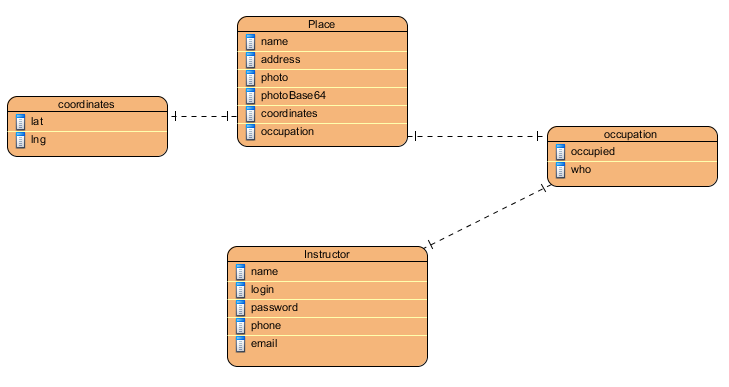
\includegraphics[width=1\textwidth]{screenshots/uml/db_schema.png}
\caption{Schemat bazy danych}
\end{figure}

Do stworzenia schematu kolekcji dokumentów bazy danych MongoDB zostało wykorzystane narzędzie typu ODM o nazwie Mongoose (patrz rozdział 2. Wykorzystywane technologie).

Listing \ref{lst:model placów} zawiera schemat bazy placów, a listing \ref{lst:model instruktorów} przedstawia schemat bazy instruktorów

\begin{lstlisting}[frame=single,label={lst:model placów},caption=Schemat danych placów manewrowych -- plik: /models/places.js]
// The Place model

var mongoose 	= require('mongoose')
  ,	Schema 		= mongoose.Schema
  ,	ObjectId 	= Schema.ObjectId
  , instructorSchema = require('./instructors');

var placeSchema = new Schema({
    place: ObjectId,
    name: String,
    address: String,
    photo: String,
    photoBase64: String,
    coordinates: {
      lat: Number,
     	lng: Number
    },
    occupation: {
        occupied: { 
          type: Boolean,
          default: false 
        },
        who: { 
          type: ObjectId,
          ref: 'Instructors'
        }
    }
});I

module.exports = mongoose.model('Place', placeSchema);
\end{lstlisting}


\begin{lstlisting}[frame=single,label={lst:model instruktorów},caption=Schemat danych instruktorów -- plik: /models/instructors.js]
// The Instructors model

var mongoose 	= require('mongoose')
  ,	Schema 		= mongoose.Schema
  ,	ObjectId 	= Schema.ObjectId;

var instructorSchema = new Schema({
    instructor: ObjectId,
    name: String,
    login: String,
    password: String,
    phone: String,  
    email: String
});

module.exports = mongoose.model('Instructors', instructorSchema);
\end{lstlisting}


\section{Panel zarządzania}

Panel zarządzania aplikacji umożliwia wykonywanie operacji CRUD (ang. Create-Read-Update-Destroy) na danych aplikacji.

Edycji użytkowników można dokonywać w obrębie \texttt{/instructors} -- jednego z~głównych kontrolerów aplikacji. A kontroler \texttt{/places} zawiera akcje odpowiedzialne za operacje na danych dotyczących placów manewrowych.


\section{Klient mobilny}

Można rozróżnić trzy sposoby wytwarzania aplikacji mobilnych, efektem których można wymienić 3 typy:
\begin{itemize}
\item aplikacje natywne,
\item aplikacje webowe,
\item aplikcje hybrydowe.
\end{itemize}

\subsubsection*{Aplikacje natywne}
To oprogramowanie tworzone najczęściej w języku programowania takim jak np.~Java, Objective-C czy C\# w zależności od platformy. Są to aplikacje pisane pod konkretny system operacyjny i mogą korzystać ze wszystkich udogodnień i funkcji sprzętowych, jakie umożliwia dane urządzenie oraz ingerować w zachowania systemu i rozszerzać jego możliwości. Są bardzo szybkie i płynne, ich interfejs może wykorzystywać systemowe UI (np. Metro w Windows Phone, Holo w Androidzie), dzięki czemu ujednolicają się doskonale z systemem, co pozwala lepiej trafić w przyzwyczajenia użytkowników. Ich największą wadą jest koszt produkcji, ponieważ, aby dotrzeć do szerszego grona odbiorców, na każdy mobilny system operacyjny musi być przygotowana oddzielna aplikacja.

\subsubsection*{Aplikacje webowe}
To nic innego jak strony internetowe zbudowane w nowych technologiach webowych, które przypominają wyglądem aplikacje mobilne. Uruchamiane są w przeglądarce internetowej i przez to wymagają ciągłego połączenia z Internetem oraz niemożliwe jest wykorzystanie w nich funkcji sprzętowych urządzenia, jakimi są m.in. aparat, kamera, GPS, żyroskop, akcelerometr. Największą i chyba jedyną zaletą tego typu aplikacji jest dostępność. Nie trzeba nic instalować, wystarczy jedynie wpisać adres internetowy aplikacji w przeglądarce internetowej, aby ją uruchomić. Aplikacje takie są uniwersalne, ponieważ maszyną uruchomieniową jest przeglądarka, więc wystarczy jeden język programowania (najczęściej jest to JavaScript), aby stworzyć uniwersalną aplikację działającą na wszystkich platformach. Co sprawia, że tego typu oprogramowanie jest stosunkowo tanie w porównaniu z aplikacjami natywnymi, gdzie nakład pracy jest o wiele większy.

\subsubsection*{Aplikacje hybrydowe}
Czyli takie jak opisywana w niniejszej pracy. Jak sama nazwa wskazuje, jest to połączenie aplikacji natywnych i webowych. Użytkownicy często nie odróżniają ich od aplikacji natywnych, jednak w sporej części budowane są w technologiach webowych takich jak HTML5, CSS3 i JavaScript, więc możliwe jest stworzenie jednej wersji oprogramowania, które działać będzie na wielu platformach. Hybrydy, tak samo jak aplikacje mobilne instalowane są w systemie i dystrybuowane w sklepach z aplikacjami takimi jak App Store czy Google Play (dawniej Android Market).
Jako, że po części napisane są w języku natywnym, a po części w webowym (wspomniane wcześniej HTML 5 czy CSS3), mają dostęp do pewnych funkcji urządzeń, na których są uruchamiane. Można wykorzystać dobrodziejstwa m.in. akcelerometru, GPS, mikrofonu, kamery, czy zapisywać i odczytywać dane z pamięci urządzenia.
Aplikacje hybrydowe umożliwiają osiągnięcie idealnej proporcji pomiędzy jakością i możliwościami aplikacji natywnych, a niskim kosztem wytwarzania aplikacji webowych.


\section{Komunikacja Klient-Serwer - API}

Dane pomiędzy klientem, a serwerem wymieniane są za pomocą protokołu JSONP (ang. JSON with padding) -- techniki komunikacyjnej umożliwiającej wykonywanie AJAX'owych zapytań do i z serwera znajdującego się w innej domenie. W normalnym przypadku taka wymiana danych nie jest możliwa ze względów bezpieczeństwa. Przeglądarki nie zezwalają na pobieranie obiektów JSON z zewnętrznego serwera w~celu zapobiegania atakom typu XSS (ang. Cross-site scripting). Udostępniają wykonywanym skryptom jedynie te obiekty, które pochodzą z tego samego źródła, co strona, w której kontekście są uruchamiane. JSONP polega na opakowaniu danych zwrotnych w funkcję typu ,,callback'', której parametr jest znany po obu stronach protokołu komunikacji, dzięki temu serwer zwraca dane jako zawartość funkcji do wywołania o takiej samej nazwie, jakiej spodziewa się klient. Kod zwrócony z serwera jest wstrzykiwany dynamicznie, a uruchomiony callback udostępnia pobrane dane do innych obiektów w przeglądarce.

Listing \ref{lst:routing-kod} zawiera routing dla wszystkich akcji udostępniających metody wymiany danych poprzez JSONP znajdujących się w kontrolerze \texttt{/api}.
Są w nim metody do pobierania list placów i instruktorów, a także do logowania.

\subsubsection*{Pobranie danych aplikacji}
Aplikacja po pomyślnym zalogowaniu pobiera listę placów i instruktorów w formacie JSON, zapisuje w lokalnej bazie danych WebSQL dostępnej w silniku renderującym WebKit wykorzystywanym w Androidzie oraz przetwarza je na interaktywne listy HTML wyświetlane jako zawartość aplikacji.

\subsubsection*{Wymiana poleceń przez API}
Każdy plac ma swój stan zajętości zapisywany w bazie i udostępniany do publicznej wiadomości pomiędzy instruktorami zalogowanymi do systemu.

Informacje o zmianach tego stanu rozpraszane są w systemie za pośrednictwem HTML5 WebSockets, który wykorzystuje biblioteka Socket.IO użyta do stworzenia oprogramowania.

W sytuacji, kiedy jeden z klientów usiłuje zająć jakiś plac, serwer otrzymuje o tym informację za pośrednictwem socketu, zapisuje do bazy danych informację o tym, że plac jest zajęty i przez kogo, w następstwie czego emituje wydarzenie, które jest propagowane do wszystkich klientów podłączonych do systemu z informacją o konieczności oznaczenia tego placu jako zajęty.

Taki stan jest utrzymywany do momentu, kiedy instruktor zwolni plac i do serwera zostanie przesłana wiadomość o zmianie stanu. Po czym serwer zmienia stan w bazie danych i rozsyła analogiczny event do wszystkich połączonych klientów, aby umożliwili od nowa zajmowanie tego placu przez innych.

Algorytm tych działań przedstawia listing \ref{lst:socket}.

Komunikacja pomiędzy socketami jest bardzo szybka, dzięki czemu w systemie nie ma opóźnień związanych z przepływem informacji.


\begin{lstlisting}[frame=single,label={lst:socket},caption=Mechanizm obsługi socketów po stronie serwera]
// Socket.IO events
io.sockets.on('connection', function (socket) {

  socket.on('placeIsOccupied', function (data) {
    places.occupyPlace(data.place, data.instructor, function(){
      io.sockets.emit('disablePlace', { place: data.place });  
    });
  });

  socket.on('placeIsFree', function (data) {
    places.releasePlace(data.place, function(){
      io.sockets.emit('enablePlace', { place: data.place });  
    });
  });

});
\end{lstlisting}

\chapter{Uruchomienie aplikacji}

\section{Aplikacja serwerowa}

Do uruchomienia aplikacji potrzebny jest interpreter Node.js. Można go pobrać ze strony projektu i zainstalować w systemie. Dostępne są dla wszystkich popularnych systemów operacyjnych. I uruchomić skrypt poleceniem \texttt{node app.js} w katalogu głównym projektu za pomocą wiersza poleceń.
Od momentu uruchomienia aplikacji, serwer będzie nasłuchiwał na określonym w konfiguracji porcie -- domyślnie jest to port \texttt{3000}.

Innym sposobem uruchomienia jest możliwość wykorzystania jednego z dostawców usług hostingowych typu PaaS (ang. Platform as a Service) takich jak np. AppFog \footnote{http://www.appfog.com/}, Heroku \footnote{https://www.heroku.com/}, czy OpenShift \footnote{https://www.openshift.com/} i uruchomienia aplikacji w chmurze jako usługa Node.js. Ta metoda jest uzależniona od wybranego usługodawcy i więcej informacji można uzyskać w dokumentacji dotyczącej tegoż hostingu.

Oprócz działającego interpretera Node.js, który będzie w stanie uruchomić aplikację, potrzebna jest jeszcze baza danych MongoDB.
Proces instalacji tego oprogramowania dla wybranych systemów operacyjnych jest szczegółowo opisany na stronie projektu \footnote{http://www.mongodb.org/}. Gdzie są też dostępne binaria instalacyjne dla najpopularniejszych systemów operacyjnych.

Najprostszym sposobem jest jednak skorzystanie z usług MongoLab \footnote{https://mongolab.com} -- platformy działającej w chmurze, umożliwiającej uruchomienie własnej instancji bazy danych MongoDB o rozmiarach do 500 MB za darmo.
Po rejestracji i stworzeniu pierwszej bazy danych, otrzymamy dane potrzebne do połączenia z bazą.

\subsubsection{Konfiguracja bazy danych}

Ważnym plikiem służącym do konfiguracji połączenia z bazą jest znajdujący się w głównym katalogu aplikacji plik \texttt{config.json}, którego zawartość należy wyedytować wstawiając do niego prawidłowe dane do połączenia.
Listing \ref{lst:dbconfig} zawiera domyślną zawartość pliku konfiguracyjnego.\\


\begin{lstlisting}[frame=single,label={lst:dbconfig},caption=Domyślna zawartość pliku z konfiguracją połączenia do bazy danych -- plik: /config.json]
{
	"mongodb": {
		"host" : "adres_serwera",
		"port" : port, // np. 3456
		"dbname" : "nazwa_bazy",
		"user" : "uzytkownik_bazy",
		"password" : "haslo_bazy"
	}
}
\end{lstlisting}


\section{Aplikacja mobilna na platformę Android}

Do uruchomienia klienta mobilnego potrzebny jest smartfon lub tablet z systemem operacyjnym Android oraz plik instalacyjny ze skompilowaną aplikacją.

Aplikacja wymaga dostępu do Internetu, aby móc komunikować się z serwerem oraz włączonego GPS, w celu liczenia odległości do placów manewrowych wyświetlanych na liście.


\subsubsection{Konfiguracja ścieżki serwera w aplikacji mobilnej}
\label{konfiguracja_adresu_serwera}

Przy pierwszym uruchomieniu zainstalowanej aplikacji pojawia się ekran wstępnej konfiguracji, w którym należy podać adres (IP, bądź domena) oraz port, na którym działa uruchomiony serwer stanowiący back-end systemu, co przedstawiają rysunki \ref{fig:ekran_poczatkowy1} (pusty formularz) oraz \ref{fig:ekran_poczatkowy2} (wypełniony danymi zgodnymi dla serwera testowego).


\begin{figure}[H]
\centering
\begin{minipage}{.48\textwidth}
  \centering
  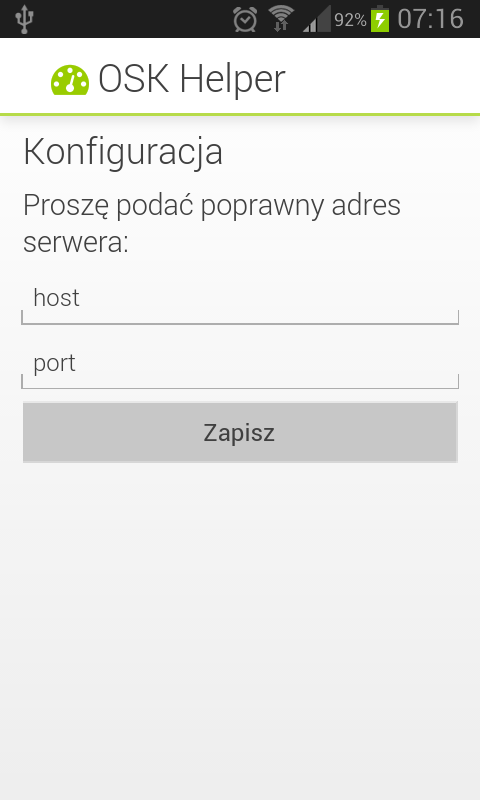
\includegraphics[width=1\linewidth]{screenshots/android/konfiguracja_serwera.png}
  %\captionof{figure}{Ekran początkowy - konfiguracja adresu serwera}
  \captionof{figure}{Konfiguracja adresu serwera - pusty formularz}
  \label{fig:ekran_poczatkowy1}
\end{minipage}%
\begin{minipage}{.04\textwidth}
   ~
\end{minipage}%
\begin{minipage}{.48\textwidth}
  \centering
  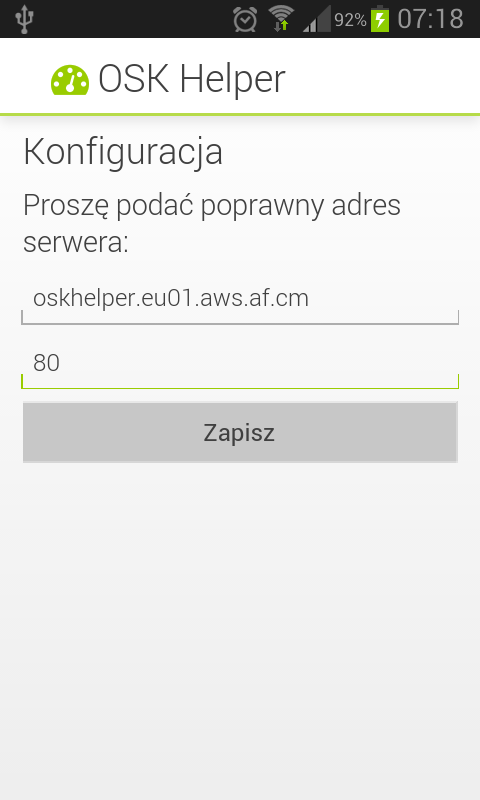
\includegraphics[width=1\linewidth]{screenshots/android/konfiguracja_serwera-wypelnione.png}
  %\captionof{figure}{Ekran początkowy - konfiguracja adresu serwera - wypełnione przykładowe dane}
  \captionof{figure}{Konfiguracja adresu serwera - wypełniony formularz}
  \label{fig:ekran_poczatkowy2}
\end{minipage}
\end{figure}

Po wprowadzeniu adresu hosta i portu aplikacja mobilna próbuje odpytać serwer pod wskazanym adresem z akcją \texttt{/api/validate\_existance}, aby sprawdzić czy wprowadzone dane są poprawne (tzw. heartbeat).

Jeśli serwer zwraca odpowiedź w formacie JSON o treści \texttt{\{'exists': true\}}, podany adres serwera jest zapisywany w pamięci aplikacji (HTML5 LocalStorage), po czym wyświetlany jest ekran logowania. Przy kolejnych uruchomieniach nie trzeba go podawać, aż do czasu wylogowania, które spowoduje wyczyszczenie lokalnej bazy danych aplikacji.


\chapter{Panel zarządzania - konfiguracja}

Panel zarządzania służy do prawidłowego skonfigurowania obiektów świata aplikacji, który ma odzwierciedlać rzeczywistość, w ramach której działa Ośrodek Szkolenia Kierowców, a w zasadzie jego pracownicy korzystający z systemu.

Możliwa jest edycja placów manewrowych i listy instruktorów z uwzględnieniem wszystkich operacji typu CRUD (ang. Create-Read-Update-Destroy). A zatem każdy z placów można edytować i usuwać, wyświetlić jego dane oraz dodać nowy plac do modelu danych aplikacji.


\newpage
\section{Zarządzanie listą placów manewrowych}

Ważne jest prawidłowe skonfigurowanie wszystkich placów, aby instruktorzy mogli z nich korzystać.

W momencie, kiedy w bazie nie ma jeszcze dodanych żadnych placów, najważniejszym ekranem jest formularz dodawania nowego placu (Rysunek \ref{fig:Nowy_plac}).

\begin{figure}[H]
\centering
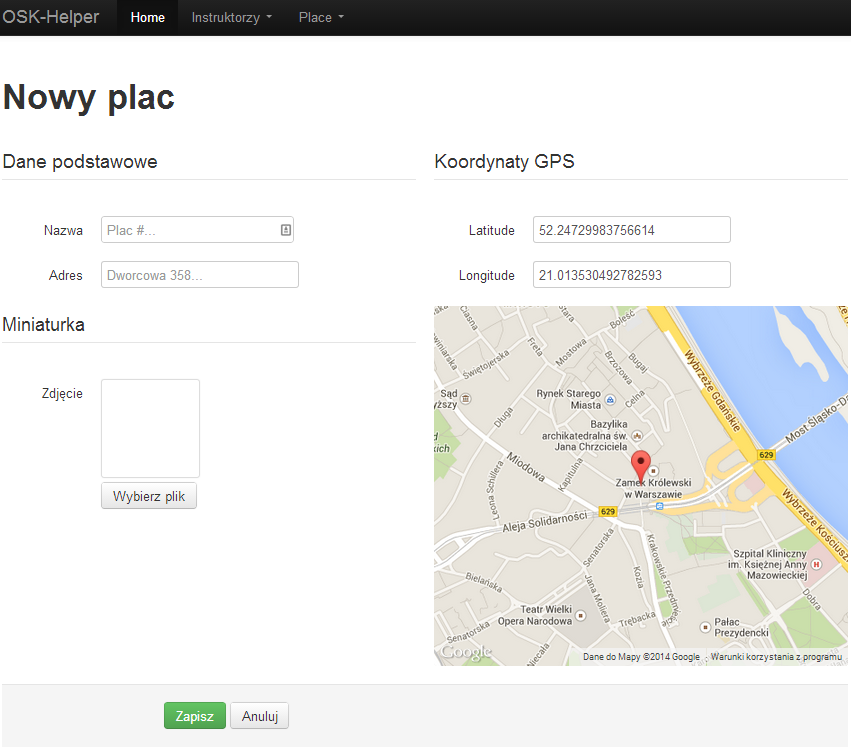
\includegraphics[width=1\textwidth]{screenshots/panel/nowy_plac.png}
\caption{Formularz dodawania nowego placu}
\label{fig:Nowy_plac}
\end{figure}

Interaktywna mapa pozwala na precyzyjne określenie współrzędnych. Pola zawierające koordynaty GPS są automatycznie uaktualniane w momencie kliknięcia w wybrany punkt na mapie.

Przesyłane na serwer zdjęcie placu jest przy okazji zapisu przetwarzane na ciąg znaków w formacie Base64  i również zapisywane do bazy danych.
Takie zdjęcie zakodowane w formie tekstowej jest przesyłane wraz z innymi danymi placów do aplikacji mobilnej, która z powrotem potrafi je wyświetlić jako obrazek i przetrzymywać w swojej lokalnej bazie danych.\newline \newline


Na rysunku \ref{fig:Lista_placow} przedstawiony jest ekran z listą, na której widoczne jest kilka pierwszych placów wprowadzonych do bazy danych. Wprowadzone dane są wygenerowane losowo przy pomocy biblioteki Faker.js \footnote{https://github.com/marak/Faker.js/}.

\begin{figure}[H]
\centering
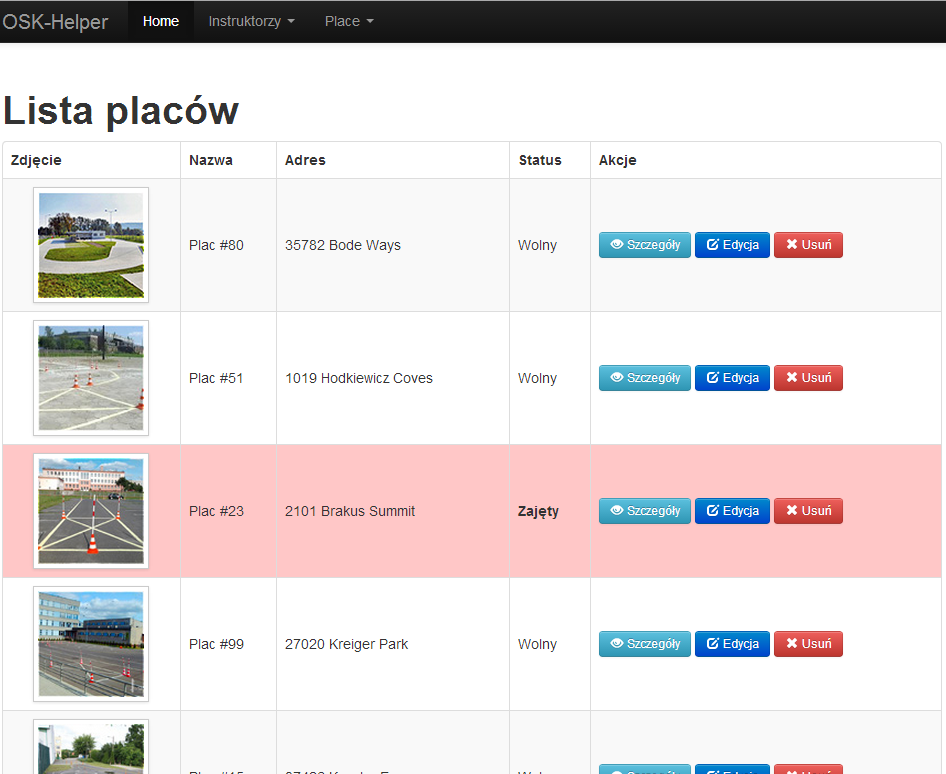
\includegraphics[width=1\textwidth]{screenshots/panel/lista_placow.png}
\caption{Lista utworzonych placów manewrowych}
\label{fig:Lista_placow}
\end{figure}

Plac o nazwie ,,Plac \#23'' na powyższym rysunku jest oznaczony jako zajęty. Wszystkie tego typu place są podświetlone wyblakłym odcieniem koloru czerwonego.

\newpage
Rysunek \ref{fig:Edycja_placu} przedstawia widok formularza do edycji danych wybranego placu.

Nie różni się on bardzo od formularza dodawania nowego placu poza tym, że ustawione aktualnie pola są już wypełnione bieżącymi danymi oraz nad częścią dotyczącą wstawiania nowego zdjęcia widnieje podgląd aktualnie wstawionej miniaturki.

Istnieje możliwość zmiany nazwy placu, adresu, współrzędnych i wgrania nowego zdjęcia.

\begin{figure}[h!]
\centering
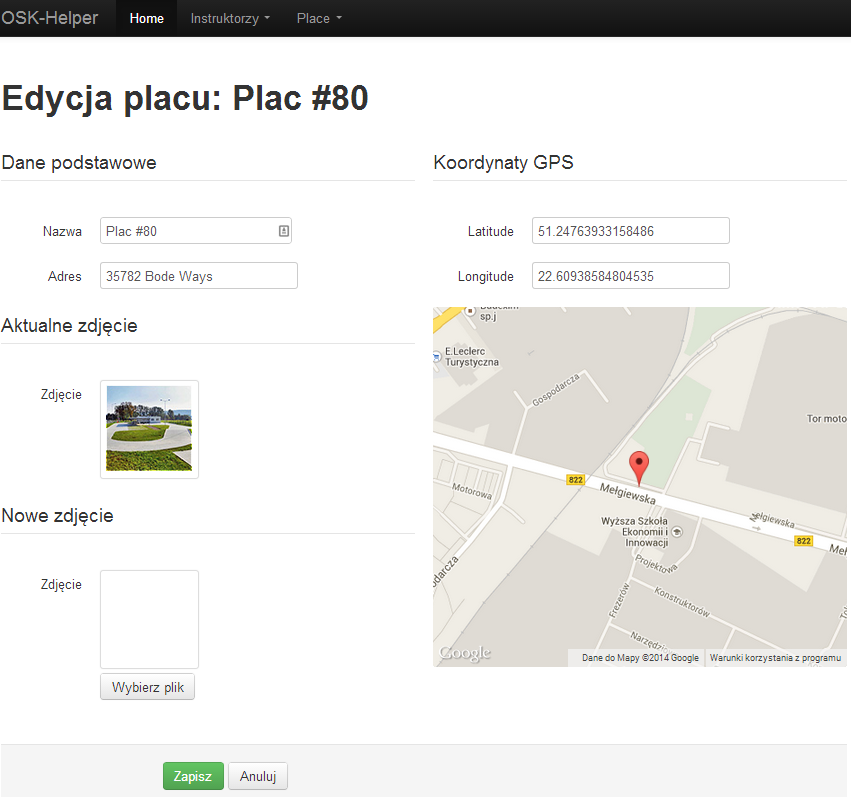
\includegraphics[width=1\textwidth]{screenshots/panel/edycja_placu.png}
\caption{Edycja wybranego placu manewrowego}
\label{fig:Edycja_placu}
\end{figure}

\newpage
\section{Zarządzanie listą instruktorów}

W przypadku konfiguracji bazy instruktorów należy postępować analogicznie.

Rysunek \ref{fig:Nowy_instruktor} przedstawia ekran z formularzem dodawania nowego instruktora. Wymienić można pola takie jak: jego nazwa osobowa, login i hasło, których będzie używał do logowania w aplikacji mobilnej oraz danych kontaktowych takich jak telefon i mail, do których wgląd będą mieli inni instruktorzy z poziomu mobilnego klienta.

\begin{figure}[H]
\centering
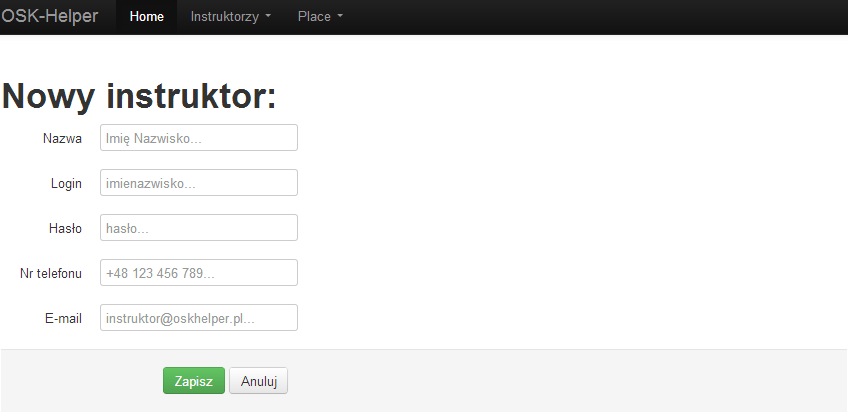
\includegraphics[width=1\textwidth]{screenshots/panel/nowy_instruktor.png}
\caption{Formularz dodawania nowego instruktora}
\label{fig:Nowy_instruktor}
\end{figure}

\newpage
Po dodaniu kilku instruktorów lista wygląda tak, jak to przedstawia rysunek \ref{fig:Nowy_instruktor}.

\begin{figure}[H]
\centering
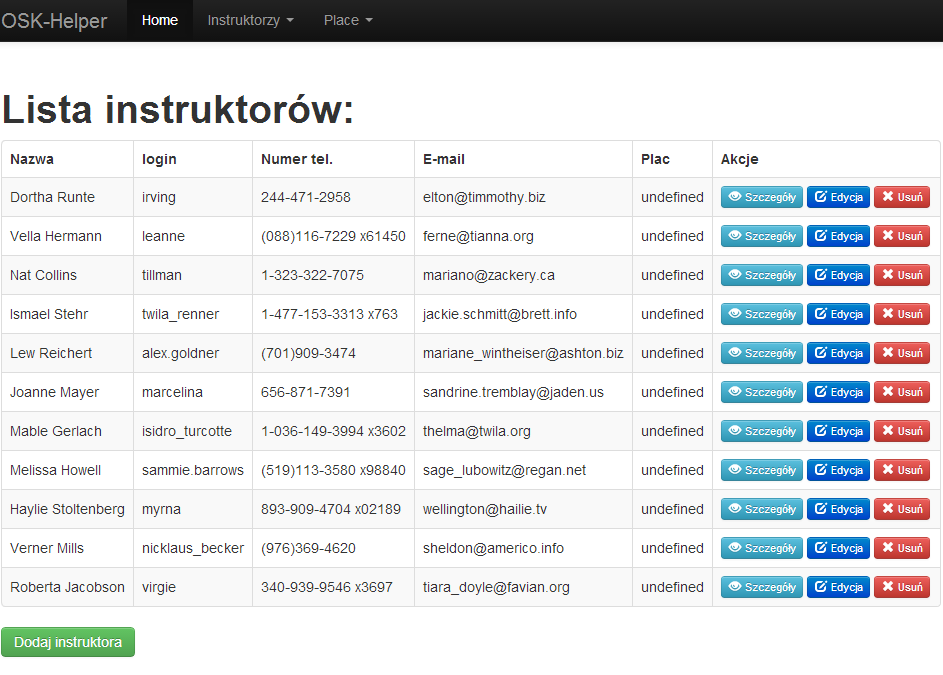
\includegraphics[width=1\textwidth]{screenshots/panel/lista_instruktorow.png}
\caption{Lista dodanych instruktorów}
\end{figure}


\chapter{Klient dla systemu Android - korzystanie}

\section{Przypadki użycia}
Rysunek \ref{fig:Diagram przypadków użycia} wizualizuje akcje możliwe do wykonania przez użytkowników aplikacji.

\begin{figure}[H]
\centering
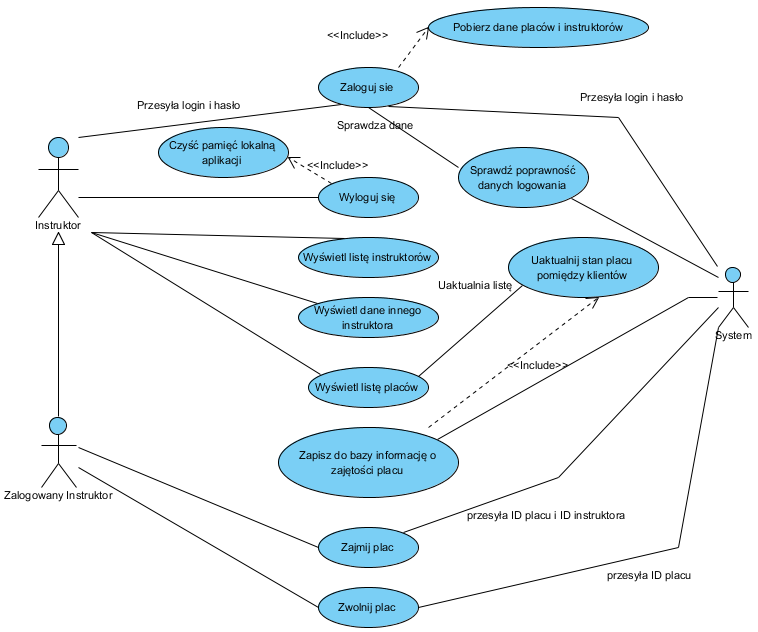
\includegraphics[width=1\textwidth]{screenshots/uml/usecases.png}
\caption{Ekran logowania użytkownika}
\label{fig:Diagram przypadków użycia}
\end{figure}


\section{Logowanie}
Aby instruktor miał możliwość korzystania z systemu, monitorowania zajętości placów oraz ingerowania w ich stan, musi być zalogowany.

Podczas pierwszego uruchomienia, tuż po poprawnym podaniu adresu serwera, pojawia się ekran logowania (rysunek \ref{fig:Logowanie_mobile}), w którym należy podać prawidłową nazwę użytkownika i hasło przypisane do instruktora.

\begin{figure}[H]
\centering
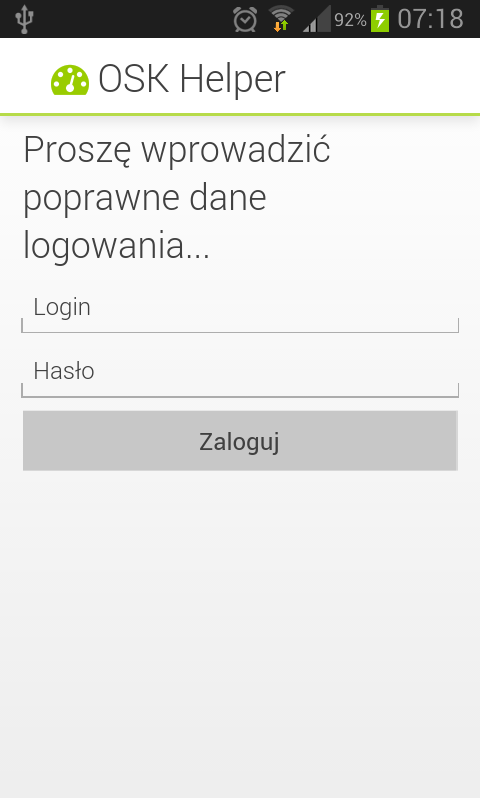
\includegraphics[width=0.5\textwidth]{screenshots/android/logowanie.png}
\caption{Ekran logowania użytkownika}
\label{fig:Logowanie_mobile}
\end{figure}

Serwer waliduje przesłany login i hasło, następnie w przypadku poprawnych danych zwraca dane umożliwiające wyrenderowanie ekranów aplikacji.


\section{Podgląd listy placów}
Domyślnym widokiem wyświetlonym po pomyślnym zalogowaniu jest lista placów.

Na podstawie położenia GPS lista jest sortowana wg odległości placów. Najbliżej położone punkty znajdują się na początku listy.

Każdy element listy zawiera nazwę placu, jego adres oraz odległość. Do obliczania odległości zostało wykorzystane Google Maps API.

Rysunek \ref{fig:Lista_placow_mobile} przedstawia ekran prezentujący listę placów.

\begin{figure}[H]
\centering
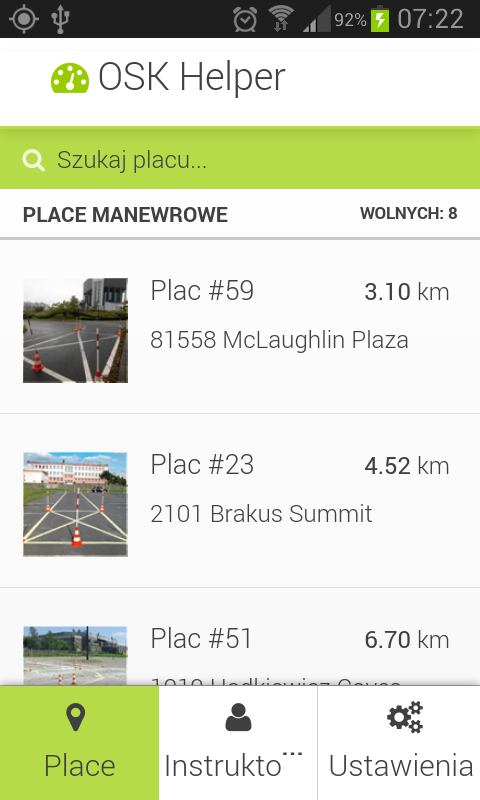
\includegraphics[width=0.5\textwidth]{screenshots/android/lista_placow.png}
\caption{Lista placów - sortowana według odległości}
\label{fig:Lista_placow_mobile}
\end{figure}

Widoczny jest na nim zielony pasek z polem wyszukiwania. Wystarczy zacząć wpisywać w nim tekst, a elementy listy dynamicznie zostają zawężane do wyników wyszukiwania wg wpisanego wzorca. Wyszukiwanie jest dokonywane zarówno w nazwie, jak i adresie placu.

Efekt wyszukiwania można zaobserwować na rysunku \ref{fig:Lista_placow-przefiltrowana_mobile}.

\begin{figure}[H]
\centering
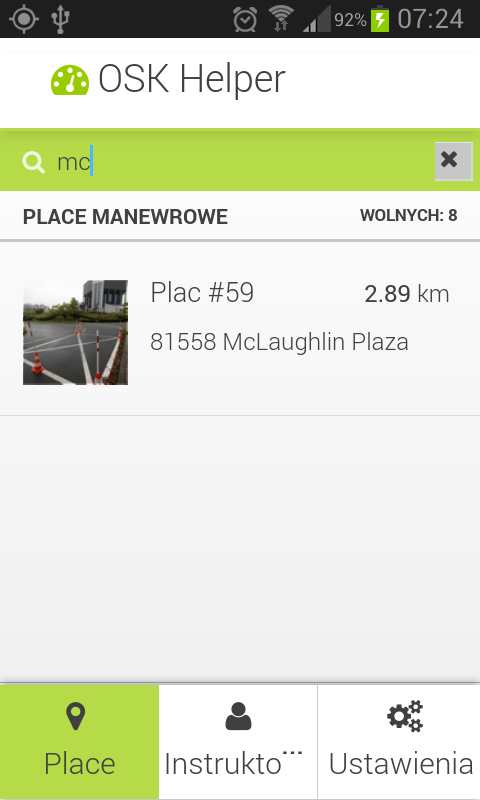
\includegraphics[width=0.5\textwidth]{screenshots/android/wyszukiwanie.png}
\caption{Lista placów - przefiltrowana wg wyszukiwanego wzorca}
\label{fig:Lista_placow-przefiltrowana_mobile}
\end{figure}


\subsection{Zajmowanie i zwalnianie placu}

Po wciśnięciu wybranego placu zostaje rozpropagowana w systemie informacja o zajętości tego placu, a użytkownik zostaje przeniesiony na ekranz  widokiem szczegółowym, który przedstawia rysunek \ref{fig:Zajmowany_plac_mobile}.

\begin{figure}[H]
\centering
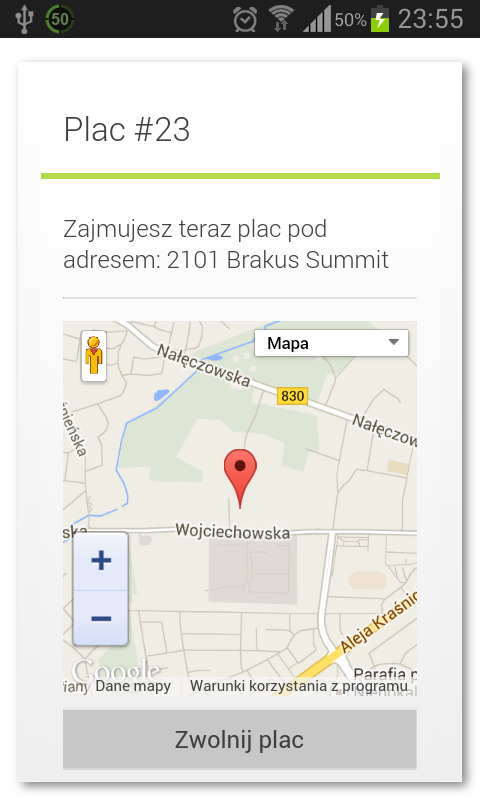
\includegraphics[width=0.7\textwidth]{screenshots/android/szczegoly_placu.png}
\caption{Widok szczegółowy zajmowanego placu}
\label{fig:Zajmowany_plac_mobile}
\end{figure}

Widoczna jest interaktywna mapa z położeniem placu, zaimplementowana z wykorzystaniem Google Maps, którą można dowolnie przybliżać, oddalać, przesuwać oraz przełączyć się na widok satelitarny lub panoramiczny.

Przycisk ,,Zwolnij plac'' pozwala wrócić do poprzedniego ekranu jednocześnie wysyłając do serwera informację o zwolnieniu placu.




\section{Podgląd listy instruktorów}

Na ekranie z listą instruktorów pracujących w ośrodku, każdy element klikalny zawiera pełną nazwę instruktora.

Widnieje na nim również wyszukiwarka działająca w sposób analogiczny do przedstawionego w części dotyczącej przeszukiwania placów.

\begin{figure}[H]
\centering
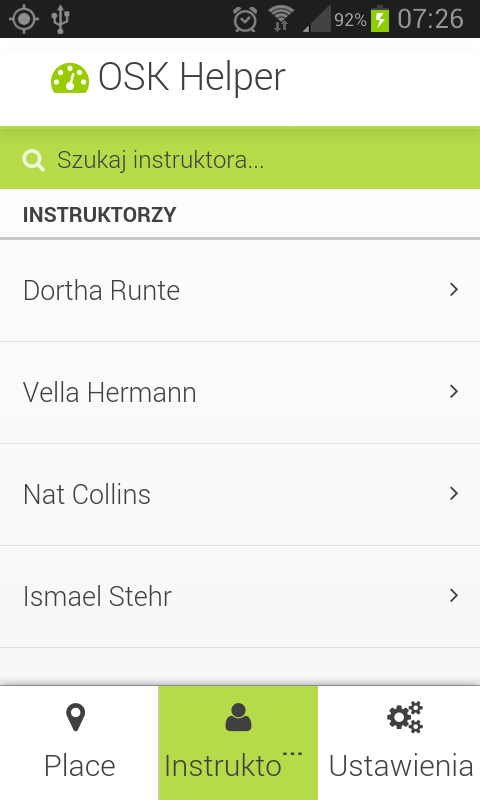
\includegraphics[width=0.4\textwidth]{screenshots/android/lista_instruktorow.png}
\caption{Lista instruktorów}
\label{fig:Lista_instruktorow_mobile}
\end{figure}

Wybranie jednego z elementu listy powoduje wyświetlenie ekranu zawierającego akcje związane z kontaktem do wybranego instruktora, co ilustruje rysunek \ref{fig:Instruktor_mobile}.

\begin{figure}[H]
\centering
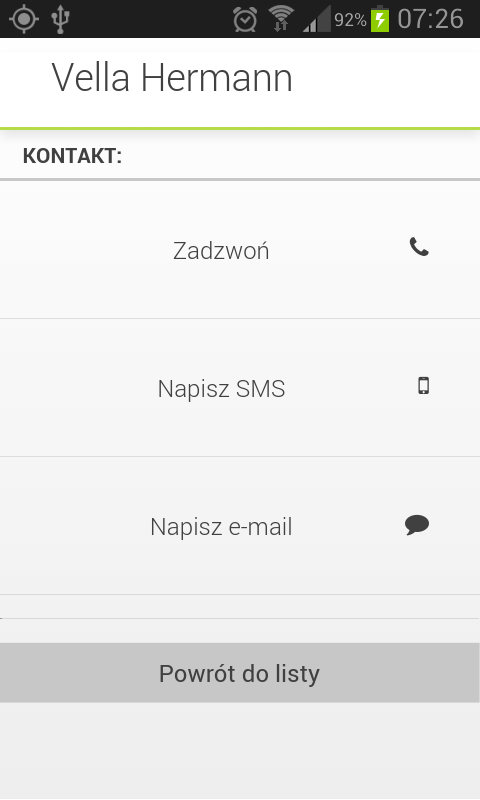
\includegraphics[width=0.4\textwidth]{screenshots/android/widok_szczegolowy_instruktora.png}
\caption{Widok szczegółowy wybranego instruktora}
\label{fig:Instruktor_mobile}
\end{figure}

Kliknięcie na konkretny przycisk powoduje wykonanie wybranej akcji z poziomu wbudowanych funkcji telefonu.

Możliwe jest wybranie numeru do przeglądanego instruktora, wysłanie wiadomości SMS lub napisanie E-maila.

\newpage
\section{Ustawienia}

Ekran ustawień umożliwia wylogowanie użytkownika.

Wyświetla również pełną nazwę zalogowanego instruktora, która zostaął skonfigurowana w panelu zarządzania.

\begin{figure}[H]
\centering
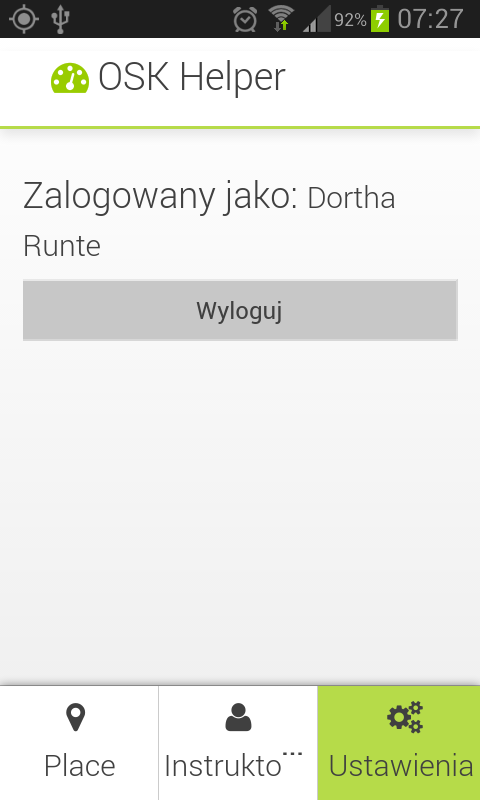
\includegraphics[width=0.5\textwidth]{screenshots/android/ustawienia.png}
\caption{Ekran ustawień - możliwość wylogowania}
\label{fig:Ustawienia_mobile}
\end{figure}

Wylogowanie powoduje wyczyszczenie całej pamięci podręcznej, więc staje się również pomocne w przypadku zmiany adresu serwera, z którym aplikacja się komunikuje. Po wylogowaniu należy od nowa wprowadzić zarówno adres serwera, jak i dane do logowania.

W przyszłości ma się tu znaleźć również możliwość zmiany hasła i wymuszenia aktualizacji.


\chapter{Podsumowanie i wnioski}

W niniejszej pracy został przedstawiony opis stworzonego systemu wspomagającego pracę instruktorów nauki jazdy.

Celem pracy było stworzenie aplikacji mobilnej na urządzenia z systemem Android, która umożliwia komunikowanie się z innymi tego typu klientami przez scentralizowany serwer napisany w technologii Node.js.

Napisana w ramach pracy aplikacja umożliwia wymianę informacji o stanach zajętości placów wprowadzonych do systemu pomiędzy klientami, ich odległości względem położenia użytkownika oraz możliwość skontaktowania się z innymi instruktorami przy pomocy wbudowanych funkcji urządzenia.

W pracy została przedstawiona architektura systemu, sposób komunikacji wewnątrz niego, instrukcja uruchomienia aplikacji oraz jej używania.

Autor napotkał na wiele trudności, które udało mu się rozwiązać, co zapewniło mu sporą dawkę doświadczenia. Praca pozwoliła autorowi na nauczenie się i zdobycie nowych umiejętności dotyczących tworzenia hybrydowych aplikacji mobilnych w technologiach webowych oraz pisania serwerów API dla nich.

Aplikacja może być w przyszłości rozwijana i wzbogacana o nowe funkcjonalności. Istnieje wiele pomysłów na dalszy rozwój i z pewnością będzie ona nadal rozwijana. Docelowo aplikacja ma stać się konkurencyjnym oprogramowaniem do zarządzania m.in. harmonogramami lekcji nauki jazdy, postępów w nauczaniu konkretnych kursantów i przydzielaniem wyposażenia instruktorów.

\backmatter

% lista rysunków
\listoffigures
% lista listingów kodu
\lstlistoflistings
% lista tabel
%\listoftables
% lista algorytmów
%\listofalgorithms

% rodzaj bibliografii
\nocite{*}
\bibliographystyle{plain}
\renewcommand{\bibname}{Literatura}
% plik z wpisami bibliograficznymi
\bibliography{bibliografia}


\end{document}
